% !TEX root = ../main.tex

% Local Variables:
% TeX-master: "../main"
% End:
% chktex-file 26

%%%%%%%%%%%%%%%%%%%%%%%%%%%%%%% Header %%%%%%%%%%%%%%%%%%%%%%%%%%%%%%%%%%%%%%%%%%%%
\begin{minipage}[l]{0.42\textwidth}
    
\includegraphics[width=1\textwidth]{img/logo-UNAMBA.png}
\end{minipage}
\hfill
\begin{minipage}[c]{0.5\textwidth}
    \begin{flushright}
	\large{\textbf{Unidad \#1}}\\
	\large{Lectures on Física I}\\
	\large{24 de Septiembre del 2025. Haquira, Apurimac}\\
        % \large{\textbf{Student:} Huallpa Aimituma Josué David}
    \end{flushright}
\end{minipage}
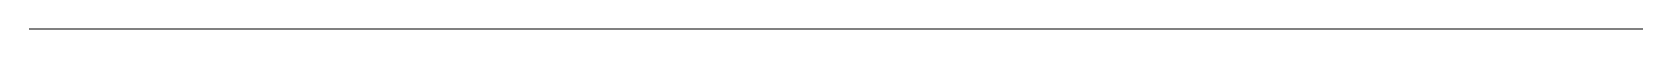
\begin{tikzpicture}
    \draw[gray,thick] (-6.5,0)--(14,0);
\end{tikzpicture}


 %%%%%%%%%%%%%%%%%%%%%%%% INICIO DEL CONTENIDO EN DOS COLUMNAS %%%%%%%%%%%%%%%%%%%%%
  
 \begin{multicols}{2}
   \begin{center}
         \LARGE{\textbf{Capítulo I: Análisis Dimensional}}\\	
         \vspace{0.2cm}
         % \Large {Lecturers Esteban Chalbaud \& Daniel Galviz} \\
         % \large{Teaching Assistant: Mauricio Gamonal \& Irvin Martínez}\\
         % \large{PhysicsLatam.com}\\
         % \vspace{0.2cm}
         \large{24 Septiembre 2025, 6:59 am (GMT-4)}\\
         % \vspace{0.2cm}
         \large{— Ficha de Trabajo —}
     \end{center}

    %  \begin{excercise}[][][$[K]=T$, $(K)=\mathrm{s}$]{ex:ad-01}{
    %        La siguiente es una fórmula física correcta
    %        \begin{equation*}
    %            K\cdot F=m\cdot v
    %        \end{equation*}
    %        donde $m=\rm{masa}$; $F=\rm{fuerza}$ y $V=\rm{velocidad}$. Determine qué magnitud representa $K$ y sus unidades en el S.I
    %      }
    % \end{excercise}
    %
    % \begin{excercise}[][][$[K]=$, $(K)=\mathrm{.}$]{ex:ad-02}{
    %        La siguiente expresión es dimesionalmente correcta y homogenea
    %        \begin{equation*}
    %            K=\frac{m\cdot v}{F\cdot t}
    %        \end{equation*}
    %        donde $m=\rm{masa}$; $F=\rm{fuerza}$; $t=\rm{tiempo}$ y $v=\rm{velocidad}$. Determine qué magnitud representa $K$ y sus unidades en el S.I
    %      }
    % \end{excercise}
    %
    % \begin{excercise}[][][$(E)=\mathrm{kg\cdot m^{-2}}$]{ex:ad-02.1}{
    %        Determinar las unidades de "E" en el sistema internacional de unidades
    %        \begin{equation*}
    %            E=\frac{\rho\cdot v^2}{g}
    %        \end{equation*}
    %        donde $\rho=\rm{densidad}$; $g=\rm{aceleración\, de\, la\, gravedad}$ y $v=\rm{velocidad}$. 
    %    }
    % \end{excercise}
    %
    % \begin{excercise}[][][$(E)=\mathrm{kg\cdot m^{-2}}$]{ex:ad-03}{
    %        Determinar las unidades de "E" en el sistema internacional de unidades
    %        \begin{equation*}
    %            E=\frac{\rho\cdot v^2}{g}
    %        \end{equation*}
    %        donde $\rho=\rm{densidad}$; $g=\rm{aceleración\, de\,  la\, gravedad}$ y $v=\rm{velocidad}$. 
    %    }
    % \end{excercise}
    %
    % \begin{excercise}[][][$[X]=LT^{-1}$, $(T)=\mathrm{ms^{-1}}$]{ex:ad-04}{
    %        La siguiente expresión es dimesionalmente correcta y homogenea, determine las dimensiones y unidades de "X"
    %        \begin{equation*}
    %            X=\omega\cdot A \cos{(\omega\cdot t+\delta)}
    %        \end{equation*}
    %        donde $A=\rm{longitud}$ y $t=\rm{tiempo}$ 
    %    }
    % \end{excercise}
    %
    % \begin{excercise}[][][$[B]=LT^{-1}$, $(B)=\mathrm{ms^{-1}}$]{ex:ad-05}{
    %        En la siguiente fórmula física, determinar la unidad de "B"
    %        \begin{equation*}
    %            a^{0.5}\cdot h^{\sin{(30^\circ)}}=B\cdot \cos{(60^\circ)}
    %        \end{equation*}
    %        donde $a=\rm{aceleración}$ y $h=\rm{altura}$
    %    }
    % \end{excercise}
    %
    % \begin{excercise}[][][$[a\cdot b]=LT$, $(a\cdot b)=\mathrm{ms}$]{ex:ad-06}{
    %        En la siguiente fórmula física, determinar la unidad de "$a\cdot b$"
    %        \begin{equation*}
    %            a=A\cdot e^{b\omega}\cdot \sin{(\omega t)}
    %        \end{equation*}
    %        donde $A=\rm{longitud}$, $t=\rm{tiempo}$
    %    }
    % \end{excercise}
    %
    % \begin{excercise}[][][$[R]=L^2$]{ex:ad-07}{
    %        En la siguiente fórmula física, ¿Qué magnitud física representa R?
    %        \begin{equation*}
    %            R=\left[\sqrt{z(h+z)}\right]\cdot\left[\frac{y}{z}-\log{x}\right]\cdot[y+A]
    %        \end{equation*}
    %        donde $h=\rm{altura}$
    %    }
    % \end{excercise}
    %
    % \begin{excercise}[][][$x+y+z=3$]{ex:ad-08}{
    %        En la siguiente fórmula física
    %        \begin{equation*}
    %            P=\rho^x\cdot Q^y\cdot h^z\cdot g
    %        \end{equation*}
    %         donde $P=\rm{potencia}$; $\rho=\rm{densidad}$; $h=\rm{altura}$; $Q=\rm{Caudad}\, (m^3/s)$;$g=\rm{aceleración\, de\, la\, gravedad}$. Hallar $x+y+z$
    %    }
    % \end{excercise}
    %
    % \begin{excercise}[][][$\displaystyle{P_h=\lambda\frac{Q^2\cdot \rho}{A^2}}$]{ex:ad-09}{
    %        La presión $P_h$ que ejerce un flujo de agua sobre una placa vertical viene dada por la siguiente fórmula empírica
    %        \begin{equation*}
    %            P_h=\lambda\cdot Q^x\cdot\rho^y\cdot g^z
    %        \end{equation*}
    %        donde $\lambda=\rm{constante\, de\, proporcionalidad}$; $\rho=\rm{densidad}$; $A=\rm{área\, de\, la\, placa}$; $Q=\rm{Caudad}\, (m^3/s)$. Determine la expresión final de la fórmula.
    %    }
    % \end{excercise}
    %
    % \begin{excercise}[][][$[R]=ML^2T^{-2}\theta^{-1}N^{-1}$, $(R)=J\cdot \rm{mol^{-1}K^{^-1}}$]{ex:ad-10}{
    %        La siguiente es la ecuación universal de los gases ideales
    %        \begin{equation*}
    %            PV=nRT
    %        \end{equation*}
    %        donde: $P=\rm{Presión}$; $V=\rm{volumen}$; $n=\rm{cantidad\, de\, sustancia}$; $T=\rm{Temperatura\, absoluta}$. Determine la dimensión de la constante de los gases ideales $R$.
    %    }
    % \end{excercise}
    %
    % \begin{excercise}[][][$[q]=I\cdot T$, $(q)=A\cdot s= \rm{1C}$]{ex:ad-11}{
    %        La intensidad de corriente eléctrica se define por la siguiente relación
    %        \begin{equation*}
    %            i=\frac{q}{t}
    %        \end{equation*}
    %        donde: $q=\rm{carga\, eléctrica}$; $t=\rm{tiempo}$. Hallar la ecuación dimensional de la carga eléctrica $q$.
    %    }
    % \end{excercise}
    %
    % \begin{excercise}[][][$[V]=M\cdot L^2\cdot T^{-3}\cdot I^{-1}$, $(V)=kg\cdot m^2\cdot s^{-3}\cdot A^{-1}= \rm{1V}$]{ex:ad-12}{
    %        Si el potencial eléctrico $V$ se define por la siguiente relación:
    %        \begin{equation*}
    %            V=\frac{W}{q}
    %        \end{equation*}
    %        donde: $q=\rm{carga\, eléctrica}$; $W=\rm{trabajo}$. Hallar la ecuación dimensional del potencial eléctrico $V$.
    %    }
    % \end{excercise}
    %
    % \begin{excercise}[][][$[C]=L^{-2}\cdot M^{-1}\cdot T^4\cdot I^2$, $(C)=\rm{m^{-2}\cdot kg^{-1}\cdot s^{4}\cdot A^{2}}= \rm{1F}$]{ex:ad-13}{
    %        La capacidad eléctrica de un condensador $C$ se define matemáticamente por la siguiente relación:
    %        \begin{equation*}
    %            C=\frac{Q}{V}
    %        \end{equation*}
    %        donde: $Q=\rm{cantidad\, de\, carga\, eléctrica}$; $V=\rm{potencial\, eléctrico}$. Hallar la ecuación dimensional de la capacidad eléctrica $C$.
    %    }
    % \end{excercise}
    %
    % \begin{excercise}[][][$[R]=L^{2}\cdot M\cdot T^{-3}\cdot I^{-2}$, $(C)=\rm{m^{2}\cdot kg\cdot s^{-3}\cdot A^{-2}}= \rm{1\Omega}$]{ex:ad-14}{
    %        La ley de Ohm, se expresa matemáticamente por la siguiente relación
    %        \begin{equation*}
    %            \Delta V=I\,R
    %        \end{equation*}
    %        donde: $\Delta V=\rm{Diferencia\, de\, potencial}$; $I=\rm{Intensidad\, de\, corriente\, eléctrica}$; $R=\rm{resistencia\, eléctrica}$. Hallar la ecuación dimensional de la resistencia eléctrica $R$.
    %    }
    % \end{excercise}
    %
    % \begin{excercise}[][][$[B]=M\cdot T^{-2}\cdot I^{-1}$, $(B)=kg\cdot s^{-2}\cdot A^{-1}= \rm{1 T}$]{ex:ad-15}{
    %        La fuerza $F$ que actúa sobre un alambre, por el cual circula una corriente $I$, está dada por la siguiente relación:
    %        \begin{equation*}
    %            F=I\,L\, B
    %        \end{equation*}
    %        donde: $B=$ densidad de flujo magnético externo o inducción magnética; $L=$ longitud del alambre. Hallar la ecuación dimensional de $B$.
    %    }
    % \end{excercise}
    %
    % \begin{excercise}[][][$[\Phi]=\rm{M\cdot L^2\cdot T^{-2}\cdot I^{-1}}$, $(\Phi)=\rm{kg\cdot ṃ^2\cdot  s^{-2}\cdot A^{-1}= \rm{1 Wb}}$]{ex:ad-16}{
    %        El flujo magnético $\Phi$  se define matemáticamente por la siguiente relación:
    %        \begin{equation*}
    %             \Phi=B\cdot A\cdot\cos{(\theta)}
    %        \end{equation*}
    %        donde: $B=$ densidad de flujo magnético; $A=$ área. Hallar la ecuación dimensional de $\Phi$.
    %    }
    % \end{excercise}
    %
    % \begin{excercise}[][][$[\mu_0]=\rm{L\cdot M\cdot T^{-2}\cdot I^{-2}}$, $(\mu_0)=\rm{m\cdot kg\cdot s^{-2}\cdot A^{-2}= \rm{1 H/m}}$]{ex:ad-17}{
    %        La densidad de flujo magnético $B$, originado por una corriente rectilinea $I$, a una distancia radial $r$, está dada por la siguiente relación: 
    %        \begin{equation*}
    %             B=\frac{\mu_0}{2\pi}\cdot\frac{1}{r}
    %        \end{equation*}
    %        Hallar la unidad en el S.I de la permeabilidad magnética $\mu_0$.
    %    }
    % \end{excercise}
 \end{multicols}
